\chapter{Wave Polarization}
\label{ch:wave-polarization}

\begin{nontechnical}
\textbf{Wave polarization is like the orientation of a jump rope}---you can shake it up/down (vertical), side-to-side (horizontal), or in circles (circular). Antennas must match this orientation to catch the signal!

\textbf{Three main types:}
\begin{itemize}
\item \textbf{Linear Polarization} (most common): Field oscillates in one fixed direction---vertical ($\updownarrow$), horizontal ($\leftrightarrow$), or slant ($\nearrow$)
\item \textbf{Circular Polarization}: Field rotates in a circle as wave travels---clockwise (RHCP) or counter-clockwise (LHCP)
\item \textbf{Elliptical Polarization}: Field traces an ellipse (in-between linear and circular)
\end{itemize}

\textbf{Real-world examples:}
\begin{itemize}
\item \textbf{FM Radio:} Vertical polarization (your car's vertical antenna must match)
\item \textbf{WiFi:} Usually vertical (tilting your laptop changes signal strength)
\item \textbf{GPS:} Circular polarization (works at any angle, survives ionospheric effects)
\end{itemize}

\textbf{Why it matters:} A 90° mismatch between transmitter and receiver polarization causes 20--30~dB signal loss---enough to drop a call or lose GPS lock. This is why your phone's GPS doesn't work well face-down on a table!
\end{nontechnical}

\section{Overview}

\textbf{Polarization} describes the \textbf{orientation of the electric field vector} as an electromagnetic wave propagates through space.

\begin{keyconcept}
While the wave travels in one direction (e.g., $+z$), the electric field \textbf{oscillates in a plane perpendicular} to propagation. The pattern traced by the $\vec{E}$-field tip defines polarization type: linear, circular, or elliptical.
\end{keyconcept}

\textbf{Why polarization matters:}
\begin{itemize}
\item \textbf{Antenna alignment:} RX antenna must match TX polarization for maximum signal capture
\item \textbf{Propagation effects:} Ionosphere rotates polarization (Faraday rotation)
\item \textbf{Interference mitigation:} Orthogonal polarizations enable frequency reuse
\item \textbf{Satellite communications:} Circular polarization combats ionospheric effects and multipath
\end{itemize}

\section{Mathematical Foundation}

\subsection{Plane Wave Representation}

The \textbf{general electric field} for a plane wave propagating in the $+z$ direction is expressed as:
\begin{equation}
\vec{E}(z,t) = E_x \cos(\omega t - kz + \phi_x)\hat{x} + E_y \cos(\omega t - kz + \phi_y)\hat{y}
\label{eq:general-efield}
\end{equation}
where:
\begin{itemize}
\item $E_x$, $E_y$ = electric field amplitudes in $x$ and $y$ directions (V/m)
\item $\omega = 2\pi f$ = angular frequency (rad/s)
\item $k = 2\pi/\lambda$ = wave number (rad/m)
\item $\phi_x$, $\phi_y$ = phase offsets (radians)
\item $\Delta\phi = \phi_y - \phi_x$ = \textbf{relative phase difference} (determines polarization type)
\end{itemize}

\textbf{At a fixed observation point} ($z = 0$):
\begin{equation}
\vec{E}(t) = E_x \cos(\omega t + \phi_x)\hat{x} + E_y \cos(\omega t + \phi_y)\hat{y}
\label{eq:efield-fixed}
\end{equation}

\begin{calloutbox}{Physical Interpretation}
The electric field vector $\vec{E}(t)$ traces a path in the $xy$-plane as time evolves. For linear polarization, this path is a straight line. For circular polarization, it's a circle. For elliptical polarization, it's an ellipse. The magnetic field $\vec{H}$ is perpendicular to both $\vec{E}$ and the direction of propagation ($\hat{z}$).
\end{calloutbox}

\section{Polarization Types}

\subsection{Linear Polarization}

\textbf{Condition:} $\Delta\phi = 0°$ or $180°$ (in-phase or anti-phase components)

\textbf{Result:} Electric field oscillates along a \textbf{fixed line} in space

\begin{equation}
\vec{E}(t) = E_0 \cos(\omega t)(\cos\theta\,\hat{x} + \sin\theta\,\hat{y})
\label{eq:linear-polarization}
\end{equation}
where $\theta$ is the angle from the horizontal axis.

\begin{center}
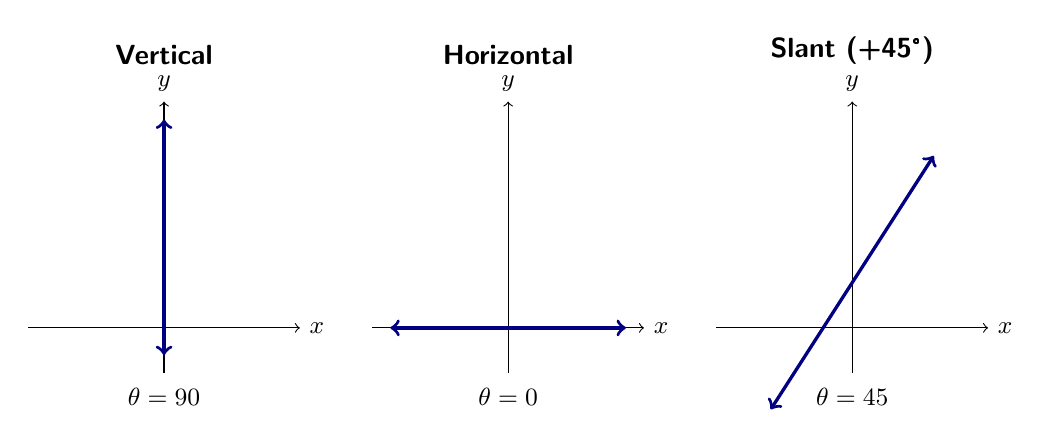
\begin{tikzpicture}[scale=1.15]
% Vertical Polarization
\begin{scope}[shift={(0,0)}]
\node[above,font=\sffamily\bfseries] at (0,2.8) {Vertical};
\draw[->] (-1.5,0) -- (1.5,0) node[right,font=\sffamily\small] {$x$};
\draw[->] (0,-0.5) -- (0,2.5) node[above,font=\sffamily\small] {$y$};
\draw[very thick,NavyBlue,<->] (0,-0.3) -- (0,2.3);
\node[below=2pt,font=\small,align=center] at (0,-0.5) {$\theta = 90°$};
\end{scope}

% Horizontal Polarization
\begin{scope}[shift={(3.8,0)}]
\node[above,font=\sffamily\bfseries] at (0,2.8) {Horizontal};
\draw[->] (-1.5,0) -- (1.5,0) node[right,font=\sffamily\small] {$x$};
\draw[->] (0,-0.5) -- (0,2.5) node[above,font=\sffamily\small] {$y$};
\draw[very thick,NavyBlue,<->] (-1.3,0) -- (1.3,0);
\node[below=2pt,font=\small,align=center] at (0,-0.5) {$\theta = 0°$};
\end{scope}

% Slant Polarization (+45°)
\begin{scope}[shift={(7.6,0)}]
\node[above,font=\sffamily\bfseries] at (0,2.8) {Slant (+45°)};
\draw[->] (-1.5,0) -- (1.5,0) node[right,font=\sffamily\small] {$x$};
\draw[->] (0,-0.5) -- (0,2.5) node[above,font=\sffamily\small] {$y$};
\draw[very thick,NavyBlue,<->] (-0.9,-0.9) -- (0.9,1.9);
\node[below=2pt,font=\small,align=center] at (0,-0.5) {$\theta = 45°$};
\end{scope}
\end{tikzpicture}
\end{center}

\subsubsection{Vertical Polarization}
\begin{equation}
\vec{E}(t) = E_0 \cos(\omega t)\hat{y}
\label{eq:vertical-pol}
\end{equation}

\textbf{E-field aligned with $y$-axis} (vertical direction)

\textbf{Applications:}
\begin{itemize}
\item AM/FM radio broadcast (vertical monopole antennas)
\item HF vertical antennas (ground wave propagation)
\item Mobile handsets (typically held vertically)
\item VHF/UHF land mobile radio
\end{itemize}

\subsubsection{Horizontal Polarization}
\begin{equation}
\vec{E}(t) = E_0 \cos(\omega t)\hat{x}
\label{eq:horizontal-pol}
\end{equation}

\textbf{E-field aligned with $x$-axis} (horizontal direction)

\textbf{Applications:}
\begin{itemize}
\item Analog TV broadcast (horizontal dipoles)
\item WiFi routers (many use horizontal dipoles)
\item Yagi antennas (horizontal for TV reception)
\end{itemize}

\subsubsection{Slant Polarization ($\pm 45°$)}
\begin{equation}
\vec{E}(t) = \frac{E_0}{\sqrt{2}} \cos(\omega t)(\hat{x} \pm \hat{y})
\label{eq:slant-pol}
\end{equation}

\textbf{E-field at $\pm 45°$ angle from horizontal}

\textbf{Applications:}
\begin{itemize}
\item Satellite polarization diversity ($+45°$ and $-45°$ as orthogonal channels)
\item Reduced building penetration loss (less reflection at oblique angles)
\item MIMO systems for decorrelation
\end{itemize}

\subsection{Circular Polarization}

\textbf{Condition:} $E_x = E_y$ and $\Delta\phi = \pm 90°$ (quadrature phase relationship)

\textbf{Result:} E-field tip traces a \textbf{circle}, rotating as the wave propagates

\begin{center}
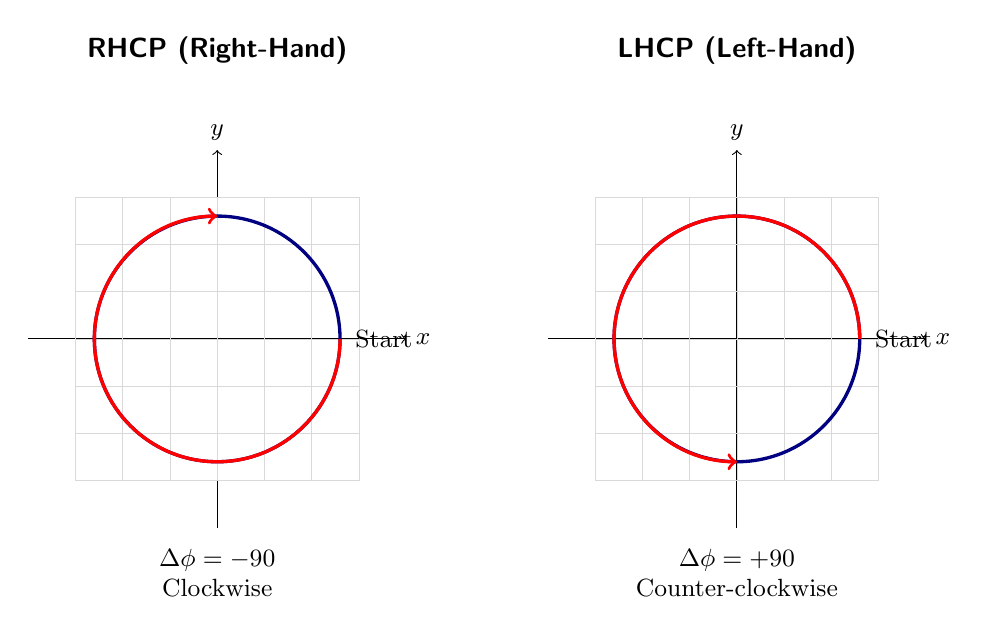
\begin{tikzpicture}[scale=1.2]
% RHCP
\begin{scope}[shift={(0,0)}]
\node[above,font=\sffamily\bfseries] at (0,2.8) {RHCP (Right-Hand)};
\draw[->] (-2,0) -- (2,0) node[right,font=\sffamily\small] {$x$};
\draw[->] (0,-2) -- (0,2) node[above,font=\sffamily\small] {$y$};
\draw[very thin,gray!30] (-1.5,-1.5) grid[step=0.5] (1.5,1.5);
\draw[very thick,NavyBlue] (0,0) circle (1.3cm);
% Rotation arrow (clockwise)
\draw[->,very thick,red] (1.3,0) arc (0:-270:1.3cm);
\node[right=2pt,font=\small] at (1.3,0) {Start};
\node[below=4pt,font=\small,align=center] at (0,-2) {$\Delta\phi = -90°$\\Clockwise};
\end{scope}

% LHCP
\begin{scope}[shift={(5.5,0)}]
\node[above,font=\sffamily\bfseries] at (0,2.8) {LHCP (Left-Hand)};
\draw[->] (-2,0) -- (2,0) node[right,font=\sffamily\small] {$x$};
\draw[->] (0,-2) -- (0,2) node[above,font=\sffamily\small] {$y$};
\draw[very thin,gray!30] (-1.5,-1.5) grid[step=0.5] (1.5,1.5);
\draw[very thick,NavyBlue] (0,0) circle (1.3cm);
% Rotation arrow (counterclockwise)
\draw[->,very thick,red] (1.3,0) arc (0:270:1.3cm);
\node[right=2pt,font=\small] at (1.3,0) {Start};
\node[below=4pt,font=\small,align=center] at (0,-2) {$\Delta\phi = +90°$\\Counter-clockwise};
\end{scope}
\end{tikzpicture}
\end{center}

\subsubsection{Right-Hand Circular Polarization (RHCP)}
\begin{equation}
\vec{E}(t) = E_0[\cos(\omega t)\hat{x} - \sin(\omega t)\hat{y}]
\label{eq:rhcp}
\end{equation}

\textbf{Viewed from receiver} (wave approaching): E-field rotates \textbf{clockwise}

\textbf{Phase relationship:} $\Delta\phi = -90°$ ($y$ component lags $x$ by $90°$)

\subsubsection{Left-Hand Circular Polarization (LHCP)}
\begin{equation}
\vec{E}(t) = E_0[\cos(\omega t)\hat{x} + \sin(\omega t)\hat{y}]
\label{eq:lhcp}
\end{equation}

\textbf{Viewed from receiver}: E-field rotates \textbf{counterclockwise}

\textbf{Phase relationship:} $\Delta\phi = +90°$ ($y$ component leads $x$ by $90°$)

\subsubsection{Properties of Circular Polarization}

\textbf{Axial ratio:} $\mathrm{AR} = 1$ (perfect circle)

\textbf{Theoretical isolation between RHCP/LHCP:} Infinite (orthogonal polarizations)

\textbf{Practical isolation:} 20--30~dB (limited by antenna imperfections)

\textbf{Applications:}
\begin{itemize}
\item \textbf{GPS satellites} (RHCP): Mitigates Faraday rotation and multipath rejection
\item \textbf{Satellite communications} (RHCP or LHCP): Reduces rain depolarization effects
\item \textbf{RFID tags}: Orientation-insensitive reading
\item \textbf{Radar systems}: Target discrimination via polarization signature
\end{itemize}

\subsection{Elliptical Polarization}

\textbf{Condition:} General case where $E_x \neq E_y$ and/or $\Delta\phi \neq 0°, 90°, 180°$

\textbf{Result:} E-field tip traces an \textbf{ellipse} in the transverse plane

The ellipse equation is:
\begin{equation}
\frac{E_x^2(t)}{A^2} + \frac{E_y^2(t)}{B^2} = 1
\label{eq:ellipse}
\end{equation}
where $A$ and $B$ are the semi-major and semi-minor axes respectively.

\begin{center}
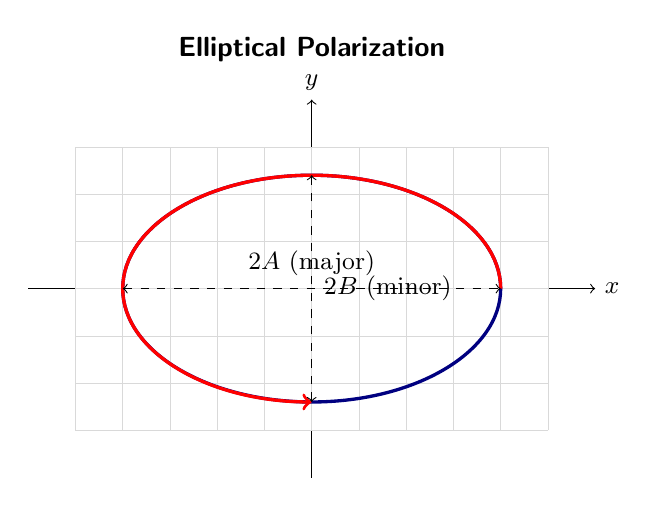
\begin{tikzpicture}[scale=1.2]
\draw[->] (-3,0) -- (3,0) node[right,font=\sffamily\small] {$x$};
\draw[->] (0,-2) -- (0,2) node[above,font=\sffamily\small] {$y$};
\draw[very thin,gray!30] (-2.5,-1.5) grid[step=0.5] (2.5,1.5);
% Ellipse
\draw[very thick,NavyBlue] (0,0) ellipse (2cm and 1.2cm);
% Rotation arrow
\draw[->,very thick,red] (2,0) arc (0:270:2cm and 1.2cm);
% Axes labels
\draw[<->,dashed] (-2,0) -- (2,0) node[midway,above=1pt,font=\small] {$2A$ (major)};
\draw[<->,dashed] (0,-1.2) -- (0,1.2) node[midway,right=1pt,font=\small] {$2B$ (minor)};
\node[above,font=\sffamily\bfseries] at (0,2.3) {Elliptical Polarization};
\end{tikzpicture}
\end{center}

\subsubsection{Axial Ratio (AR)}

The \textbf{axial ratio} quantifies the eccentricity of the ellipse:
\begin{equation}
\mathrm{AR} = \frac{\text{Major axis}}{\text{Minor axis}} = \frac{A}{B}
\label{eq:axial-ratio}
\end{equation}

\textbf{In decibels:}
\begin{equation}
\mathrm{AR}_{\text{dB}} = 20\log_{10}\left(\frac{A}{B}\right)
\label{eq:axial-ratio-db}
\end{equation}

\textbf{Special cases:}
\begin{itemize}
\item $\mathrm{AR} = 1$ (0~dB): Perfect circular polarization
\item $\mathrm{AR} \to \infty$ ($\infty$~dB): Linear polarization
\item $\mathrm{AR} < 3$~dB: Typically specified for ``circular'' antennas (acceptable ellipticity)
\end{itemize}

\subsubsection{Sense of Rotation}

\textbf{Right-hand elliptical (RHEP):} Rotates clockwise when viewed from receiver

\textbf{Left-hand elliptical (LHEP):} Rotates counterclockwise when viewed from receiver

\begin{calloutbox}{Example: Elliptical Polarization}
Consider $E_x = 2E_0$ and $E_y = E_0$ with $\Delta\phi = 90°$:
\begin{itemize}
\item Polarization is \textbf{elliptical} (not circular due to unequal amplitudes)
\item Sense of rotation: \textbf{Right-hand} ($90°$ phase relationship like RHCP)
\item Axial ratio: $\mathrm{AR} = 2E_0/E_0 = 2$ (6~dB)
\end{itemize}
\end{calloutbox}

\section{Polarization Loss Factor (PLF)}

\textbf{Mismatch between transmitter and receiver polarizations causes signal loss.} The polarization loss factor quantifies this effect:
\begin{equation}
\mathrm{PLF} = |\hat{e}_{\text{TX}} \cdot \hat{e}_{\text{RX}}^*|^2
\label{eq:plf}
\end{equation}
where $\hat{e}$ represents normalized polarization vectors (complex notation).

\subsection{Linear Polarization Mismatch}

For two linearly polarized antennas with angular mismatch $\theta$:
\begin{equation}
\mathrm{PLF} = \cos^2\theta
\label{eq:plf-linear}
\end{equation}

\textbf{Polarization loss in decibels:}
\begin{equation}
L_{\text{pol}} = -10\log_{10}(\cos^2\theta) = -20\log_{10}(\cos\theta)
\label{eq:pol-loss-db}
\end{equation}

\textbf{Examples:}

\begin{center}
\begin{tabular}{@{}crc@{}}
\toprule
\textbf{Angle Mismatch} & \textbf{Loss (dB)} & \textbf{Meaning} \\
\midrule
$0°$ & 0~dB & Perfect match \\
$30°$ & 1.2~dB & Minor loss \\
$45°$ & 3.0~dB & Half power \\
$60°$ & 6.0~dB & Quarter power \\
$90°$ & $\infty$~dB & Complete null (orthogonal) \\
\bottomrule
\end{tabular}
\end{center}

\subsection{Circular Polarization Mismatch}

\begin{center}
\begin{tabular}{@{}llcc@{}}
\toprule
\textbf{TX Polarization} & \textbf{RX Polarization} & \textbf{PLF} & \textbf{Loss (dB)} \\
\midrule
RHCP & RHCP & 1 & 0 (co-pol) \\
LHCP & LHCP & 1 & 0 (co-pol) \\
RHCP & LHCP & 0 & $\infty$ (cross-pol) \\
LHCP & RHCP & 0 & $\infty$ (cross-pol) \\
\bottomrule
\end{tabular}
\end{center}

\textbf{Terminology:}
\begin{itemize}
\item \textbf{Co-polarized:} Same sense (RHCP--RHCP or LHCP--LHCP)
\item \textbf{Cross-polarized:} Opposite sense (RHCP--LHCP or LHCP--RHCP)
\end{itemize}

\subsection{Linear to Circular Mismatch}

When a linear antenna receives a circularly polarized wave (or vice versa):
\begin{equation}
\mathrm{PLF} = 0.5 \quad \Rightarrow \quad L_{\text{pol}} = -3\ \text{dB}
\label{eq:lin-circ-loss}
\end{equation}

\begin{calloutbox}{Physical Interpretation}
A linear antenna captures only one component (e.g., horizontal or vertical) of the circular wave. Since a circular wave has equal power in both components, the linear antenna receives exactly half the available power---hence the 3~dB loss.
\end{calloutbox}

\textbf{Example:} GPS receiver with linear patch antenna
\begin{itemize}
\item GPS satellites transmit RHCP
\item Linear patch antenna: 3~dB polarization loss
\item Requires higher antenna gain or lower noise figure to compensate
\end{itemize}

\section{Polarization Generation}

\subsection{Linear Polarization}

\textbf{Simple dipole or monopole antenna:}
\begin{itemize}
\item Current flows in one direction $\Rightarrow$ E-field perpendicular to current
\item Vertical monopole $\Rightarrow$ Vertical polarization
\item Horizontal dipole $\Rightarrow$ Horizontal polarization
\end{itemize}

The polarization direction is always perpendicular to the antenna element orientation.

\subsection{Circular Polarization}

\subsubsection{Crossed Dipoles with $90°$ Phase Shift}

\textbf{Configuration:} Two perpendicular dipoles fed with:
\begin{itemize}
\item Equal amplitude currents
\item $90°$ phase difference (quadrature)
\end{itemize}

\textbf{Feed currents:}
\begin{align}
I_x &= I_0 \cos(\omega t) \label{eq:ix-feed} \\
I_y &= I_0 \cos(\omega t - 90°) = I_0 \sin(\omega t) \label{eq:iy-feed}
\end{align}

\textbf{Result:} RHCP (assuming correct phase relationship)

\textbf{Implementation:} $90°$ hybrid coupler (branch-line or Lange coupler)

\subsubsection{Helical Antenna}

\textbf{Geometry:} Helix wound around cylinder (axial mode operation)
\begin{itemize}
\item Diameter: $D \approx \lambda/\pi$ (circumference $\approx \lambda$)
\item Pitch angle: $12°$--$15°$
\item Number of turns: 5--10 for good axial ratio
\end{itemize}

\textbf{Result:} Circular polarization with sense determined by helix direction:
\begin{itemize}
\item Right-hand helix $\Rightarrow$ RHCP
\item Left-hand helix $\Rightarrow$ LHCP
\end{itemize}

\textbf{Applications:} GPS antennas, satellite ground stations, amateur radio

\subsubsection{Patch Antenna with Corner Truncation}

\textbf{Configuration:} Circular or square patch with two opposite corners truncated

\textbf{Mechanism:} Corner truncation creates two orthogonal resonant modes with approximately $90°$ phase difference

\textbf{Result:} Circular polarization (RHCP or LHCP depending on which corners are cut)

\textbf{Applications:} GPS receivers, compact GNSS antennas, mobile satellite terminals

\section{Propagation Effects on Polarization}

\subsection{Faraday Rotation}

The \textbf{ionosphere causes polarization rotation} due to the interaction of electromagnetic waves with free electrons in Earth's magnetic field. For linear polarization, this results in a rotated linear polarization.

\textbf{Faraday rotation angle:}
\begin{equation}
\Omega = 2.36 \times 10^4 \frac{B_\parallel \cdot \mathrm{TEC}}{f^2} \quad \text{(radians)}
\label{eq:faraday-rotation}
\end{equation}
where:
\begin{itemize}
\item $B_\parallel$ = Earth's magnetic field component along propagation path (Tesla)
\item $\mathrm{TEC}$ = Total Electron Content (electrons/m$^2$)
\item $f$ = frequency (Hz)
\end{itemize}

\textbf{Key observation:} Effect scales as $1/f^2$ (severe at HF, negligible at SHF)

\begin{warningbox}
\textbf{HF Example:} At 10~MHz with TEC $= 10^{18}$~el/m$^2$:
\begin{itemize}
\item Rotation: $\sim 500°$ (multiple full rotations!)
\item Linear polarization becomes \textbf{unusable} (unpredictable rotation)
\end{itemize}
\end{warningbox}

\textbf{Mitigation:} Use \textbf{circular polarization}---completely immune to Faraday rotation because rotation of circular polarization remains circular with the same sense.

\subsection{Rain Depolarization}

\textbf{Rain causes differential attenuation} between horizontal and vertical components due to the oblate shape of raindrops (wider than tall).

\textbf{Effect on polarization:}
\begin{itemize}
\item Linear $\Rightarrow$ Elliptical (unequal H and V attenuation)
\item Circular $\Rightarrow$ Elliptical (degrades axial ratio)
\end{itemize}

\textbf{Cross-Polarization Discrimination (XPD):}
\begin{equation}
\mathrm{XPD} = \frac{P_{\text{co-pol}}}{P_{\text{cross-pol}}} \quad \text{(dB)}
\label{eq:xpd}
\end{equation}

\textbf{Typical values:}
\begin{itemize}
\item Clear air: 30~dB isolation between orthogonal polarizations
\item Heavy rain: 15--20~dB isolation (increased cross-polarization interference)
\end{itemize}

\textbf{Example:} Satellite Ku-band with $\pm 45°$ linear polarization
\begin{itemize}
\item Clear weather: 30~dB isolation between $+45°$ and $-45°$ channels
\item Heavy rain (40~mm/hr): 20~dB isolation $\Rightarrow$ increased interference
\end{itemize}

\textbf{Mitigation strategies:}
\begin{itemize}
\item Adaptive coding and modulation (ACM)
\item Switch to single polarization during heavy rain
\item Increase link margin to account for depolarization
\end{itemize}

\subsection{Reflection at Surfaces}

\subsubsection{Normal Incidence}

For perpendicular incidence on a good conductor:
\begin{itemize}
\item Both horizontal and vertical polarizations reflect with $180°$ phase shift
\item Polarization type preserved (linear remains linear, circular remains circular but with opposite sense)
\end{itemize}

\subsubsection{Oblique Incidence and Brewster's Angle}

\textbf{Brewster angle} $\theta_B$ is the angle of incidence at which parallel-polarized (p-polarized) light experiences zero reflection:
\begin{equation}
\theta_B = \arctan\left(\frac{n_2}{n_1}\right)
\label{eq:brewster-angle}
\end{equation}

\textbf{Example:} Air-to-glass interface ($n_1 = 1$, $n_2 = 1.5$)
\begin{equation}
\theta_B = \arctan(1.5) \approx 56°
\label{eq:brewster-example}
\end{equation}

\textbf{Applications:}
\begin{itemize}
\item Polarizing filters (sunglasses, camera filters)
\item Anti-reflection coatings
\item Laser cavity windows (Brewster windows)
\end{itemize}

\section{Applications}

\subsection{Satellite Communications}

\textbf{Frequency reuse via polarization diversity} enables doubling channel capacity:

\textbf{Traditional approach:} Horizontal and vertical (or $\pm 45°$ linear)
\begin{itemize}
\item Two independent channels on same frequency
\item Isolation: 25--30~dB (limited by cross-polarization)
\end{itemize}

\textbf{Modern approach:} RHCP and LHCP
\begin{itemize}
\item Better rain performance (less depolarization)
\item Isolation: 20--30~dB
\end{itemize}

\begin{calloutbox}{Example: Ku-Band Direct Broadcast Satellite (DBS)}
\begin{itemize}
\item Frequency: 12~GHz downlink
\item Odd transponders: RHCP
\item Even transponders: LHCP
\item Result: \textbf{Double capacity} on same spectrum allocation
\end{itemize}
\end{calloutbox}

\subsection{GPS and GNSS}

\textbf{All GPS satellites transmit RHCP} for three critical reasons:

\begin{enumerate}
\item \textbf{Faraday rotation immunity:} Circular polarization is unaffected by ionospheric rotation
\item \textbf{Multipath rejection:} Ground reflection flips RHCP $\Rightarrow$ LHCP, which is rejected by the receiver (20--30~dB isolation)
\item \textbf{Orientation insensitive:} Works at any receiver angle within the hemisphere
\end{enumerate}

\textbf{Receiver antenna types:}
\begin{itemize}
\item RHCP patch antenna (most common in consumer devices)
\item Helical antenna (professional surveying equipment)
\item Quadrifilar helix (compact mobile applications)
\end{itemize}

\subsection{Polarimetric Radar}

\textbf{Polarimetric radar} transmits and receives multiple polarizations to extract target information:

\textbf{Measurement modes:}
\begin{itemize}
\item \textbf{HH:} Transmit H, receive H (co-polarized horizontal)
\item \textbf{VV:} Transmit V, receive V (co-polarized vertical)
\item \textbf{HV:} Transmit H, receive V (cross-polarized)
\item \textbf{VH:} Transmit V, receive H (cross-polarized)
\end{itemize}

\textbf{Applications:}
\begin{itemize}
\item \textbf{Weather radar:} Distinguish rain, hail, snow by depolarization signature
\item \textbf{SAR imaging:} Surface classification (vegetation vs metal vs water)
\item \textbf{Military radar:} Target identification (vehicles vs trees vs terrain)
\end{itemize}

\subsection{WiFi and Cellular MIMO}

\textbf{Diversity antennas} use orthogonal polarizations to improve performance:

\textbf{MIMO systems} (2$\times$2, 4$\times$4) employ $\pm 45°$ slant polarization:
\begin{itemize}
\item Reduces correlation between antenna elements
\item Improves capacity in rich scattering environments
\item Provides spatial diversity for fading mitigation
\end{itemize}

\begin{calloutbox}{Example: WiFi 802.11ac Router}
\begin{itemize}
\item Antenna 1: $+45°$ slant polarization
\item Antenna 2: $-45°$ slant polarization
\item Independent fading channels $\Rightarrow$ Diversity gain
\item Improved throughput in multipath environments
\end{itemize}
\end{calloutbox}

\subsection{EMI/EMC Testing}

\textbf{Electromagnetic compatibility standards} (FCC, CISPR) require emissions testing at both horizontal and vertical polarizations to identify worst-case emissions:
\begin{itemize}
\item Rotate receiving antenna through both polarizations
\item Measure peak emissions in each orientation
\item Report maximum measured level regardless of polarization
\end{itemize}

\section{Stokes Parameters and Poincaré Sphere}

The \textbf{Stokes parameters} provide a complete mathematical description of polarization state, including both intensity and polarization characteristics:
\begin{align}
S_0 &= E_x^2 + E_y^2 \quad \text{(total intensity)} \label{eq:stokes-s0} \\
S_1 &= E_x^2 - E_y^2 \quad \text{(H vs V preference)} \label{eq:stokes-s1} \\
S_2 &= 2E_xE_y\cos\Delta\phi \quad \text{($\pm 45°$ preference)} \label{eq:stokes-s2} \\
S_3 &= 2E_xE_y\sin\Delta\phi \quad \text{(circular preference)} \label{eq:stokes-s3}
\end{align}

\textbf{Interpretation:}
\begin{itemize}
\item $S_3 > 0$: Right-hand (RHCP) dominant
\item $S_3 < 0$: Left-hand (LHCP) dominant
\item $S_3 = 0$: Linear polarization
\end{itemize}

\textbf{Degree of polarization:}
\begin{equation}
\mathrm{DOP} = \frac{\sqrt{S_1^2 + S_2^2 + S_3^2}}{S_0}
\label{eq:dop}
\end{equation}
where DOP ranges from 0 (completely unpolarized) to 1 (fully polarized).

\subsection{Poincaré Sphere Representation}

The \textbf{Poincaré sphere} provides an intuitive 3D visualization of all possible polarization states:

\begin{center}
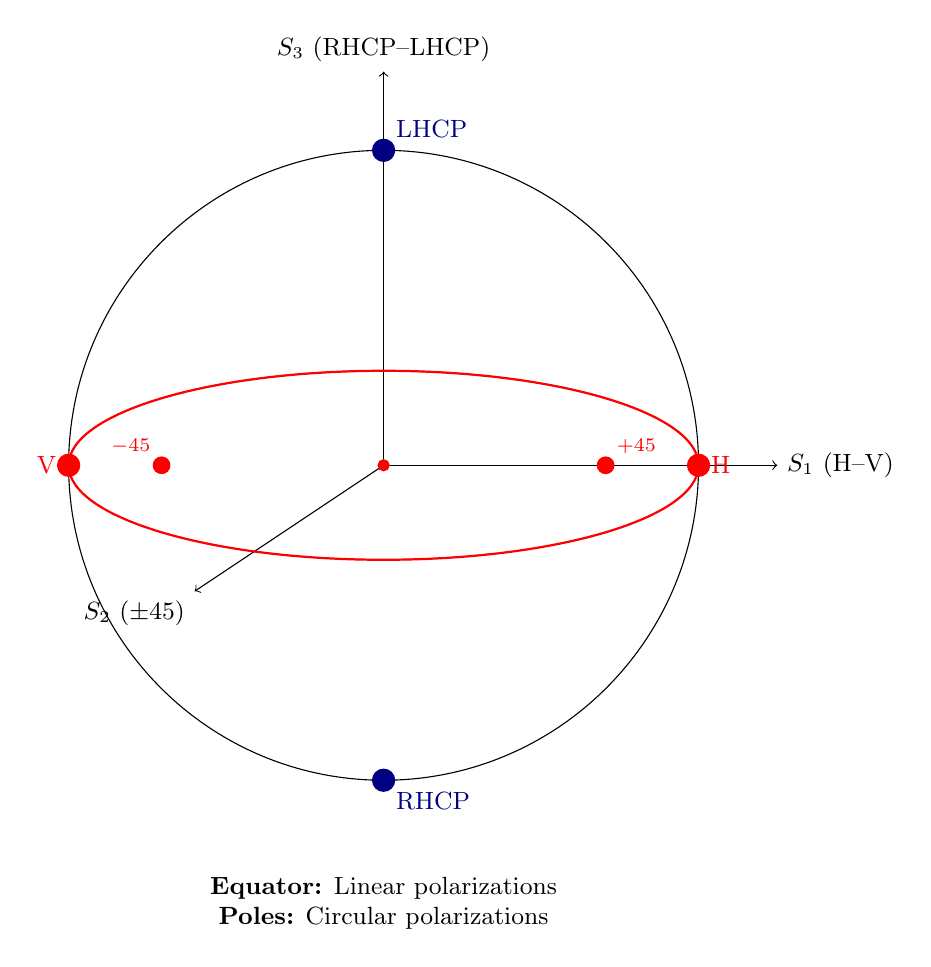
\begin{tikzpicture}[scale=2]
% Draw sphere
\draw (0,0) circle (2cm);
\draw[dashed] (-2,0) arc (180:360:2cm and 0.6cm);
\draw (2,0) arc (0:180:2cm and 0.6cm);

% Axes
\draw[->] (0,0) -- (2.5,0) node[right,font=\small] {$S_1$ (H--V)};
\draw[->] (0,0) -- (0,2.5) node[above,font=\small] {$S_3$ (RHCP--LHCP)};
\draw[->] (0,0) -- (-1.2,-0.8) node[below left,font=\small] {$S_2$ ($\pm 45°$)};

% Poles
\filldraw[NavyBlue] (0,2) circle (2pt) node[above right=1pt,font=\small] {LHCP};
\filldraw[NavyBlue] (0,-2) circle (2pt) node[below right=1pt,font=\small] {RHCP};

% Equator points
\filldraw[red] (2,0) circle (2pt) node[right=1pt,font=\small] {H};
\filldraw[red] (-2,0) circle (2pt) node[left=1pt,font=\small] {V};
\filldraw[red] (0,0) circle (1pt);
\filldraw[red] (1.41,0) circle (1.5pt) node[above right=0.5pt,font=\scriptsize] {$+45°$};
\filldraw[red] (-1.41,0) circle (1.5pt) node[above left=0.5pt,font=\scriptsize] {$-45°$};

% Equator line
\draw[red,thick] (0,0) ellipse (2cm and 0.6cm);

\node[below=3pt,font=\small,align=center] at (0,-2.5) {\textbf{Equator:} Linear polarizations\\\textbf{Poles:} Circular polarizations};
\end{tikzpicture}
\end{center}

\textbf{Key features:}
\begin{itemize}
\item \textbf{North pole ($S_3 = +1$):} LHCP
\item \textbf{South pole ($S_3 = -1$):} RHCP  
\item \textbf{Equator ($S_3 = 0$):} All linear polarizations (H, V, $\pm 45°$)
\item \textbf{Intermediate points:} Elliptical polarizations
\end{itemize}

\textbf{Applications:} Visualizing polarization transformations (e.g., Faraday rotation appears as rotation around the $S_3$ axis)

\section{Worked Example: Polarization Mismatch Analysis}

\textbf{Scenario:} Calculate the received power loss for a misaligned antenna system

\subsection*{Given Parameters}

\noindent
\begin{tabular}{@{}ll@{}}
Transmitter power & $P_t = 10$~W = 40~dBm \\
Transmitter antenna gain & $G_t = 15$~dBi (vertical polarization) \\
Receiver antenna gain & $G_r = 12$~dBi (slant $30°$ from vertical) \\
Free-space path loss & $L_{\text{FSPL}} = 120$~dB \\
Other losses & $L_{\text{other}} = 3$~dB \\
\end{tabular}

\subsection*{Step 1: Calculate Polarization Mismatch Angle}

The transmitter uses vertical polarization ($\theta_{\text{TX}} = 90°$) and the receiver is slanted at $30°$ from vertical ($\theta_{\text{RX}} = 60°$).

Angular mismatch:
\begin{equation}
\theta = |\theta_{\text{TX}} - \theta_{\text{RX}}| = |90° - 60°| = 30°
\end{equation}

\subsection*{Step 2: Calculate Polarization Loss}

Using \Cref{eq:pol-loss-db}:
\begin{equation}
L_{\text{pol}} = -20\log_{10}(\cos 30°) = -20\log_{10}(0.866) = 1.25~\text{dB}
\end{equation}

\subsection*{Step 3: Link Budget Calculation}

Total received power:
\begin{align}
P_r &= P_t + G_t + G_r - L_{\text{FSPL}} - L_{\text{pol}} - L_{\text{other}} \\
&= 40 + 15 + 12 - 120 - 1.25 - 3 \\
&= -57.25~\text{dBm}
\end{align}

\subsection*{Step 4: Impact Assessment}

\textbf{Comparison:} If polarizations were perfectly matched ($\theta = 0°$):
\begin{equation}
P_r^{\text{matched}} = 40 + 15 + 12 - 120 - 0 - 3 = -56~\text{dBm}
\end{equation}

\textbf{Result:} The $30°$ polarization mismatch causes \textbf{1.25~dB additional loss}, reducing received power from $-56$~dBm to $-57.25$~dBm.

\begin{calloutbox}[colback=black!8!white,colframe=black]{Practical Interpretation}
A 1.25~dB loss may seem small, but in a margin-limited link:
\begin{itemize}
\item Reduces effective range by approximately 15\%
\item May push BER above acceptable threshold
\item Could cause intermittent dropouts in mobile scenarios
\end{itemize}

\textbf{Lesson:} Proper antenna alignment is critical for optimal performance.
\end{calloutbox}

\section{Polarization Measurement Techniques}

\subsection{Axial Ratio Measurement}

\textbf{For circular polarization antennas:}

\textbf{Method 1---Spinning Linear Antenna:}
\begin{enumerate}
\item Rotate a linear receiving antenna through $360°$
\item Measure maximum power $P_{\text{max}}$ and minimum power $P_{\text{min}}$
\item Calculate axial ratio:
\begin{equation}
\mathrm{AR}_{\text{dB}} = 10\log_{10}\left(\frac{P_{\text{max}}}{P_{\text{min}}}\right)
\label{eq:ar-measurement}
\end{equation}
\end{enumerate}

\textbf{Method 2---Dual-Polarization Receiver:}
\begin{enumerate}
\item Measure $E_x$ and $E_y$ amplitudes and relative phase
\item Calculate AR from ellipse semi-axes
\item More accurate but requires phase-coherent receiver
\end{enumerate}

\textbf{Specification:} Good circular antenna has AR $< 3$~dB

\subsection{Cross-Polarization Discrimination}

\textbf{For linear polarization antennas:}
\begin{equation}
\mathrm{XPD} = \frac{P_{\text{co-pol}}}{P_{\text{cross-pol}}} \quad \text{(dB)}
\end{equation}

\textbf{Typical values:}
\begin{itemize}
\item Well-designed antenna: XPD $> 25$~dB
\item Practical systems: XPD $\approx 20$--30~dB
\end{itemize}

\section{Practical Considerations}

\subsection{Bandwidth Limitations}

\textbf{Circular polarization antennas are inherently narrowband:}
\begin{itemize}
\item The $90°$ phase shift is frequency-dependent
\item Typical fractional bandwidth: 2--5\% for AR $< 3$~dB
\item Wideband circular polarization requires complex feed networks
\end{itemize}

\subsection{Cost and Complexity Trade-offs}

\begin{center}
\begin{tabular}{@{}llll@{}}
\toprule
\textbf{Polarization} & \textbf{Complexity} & \textbf{Cost} & \textbf{Typical Applications} \\
\midrule
Linear & Simple & Low & AM/FM, WiFi, cellular \\
Circular & Moderate & Medium & GPS, satellite, RFID \\
Dual-polarized & High & High & Radar, satellite (frequency reuse) \\
\bottomrule
\end{tabular}
\end{center}

\section{Summary}

\begin{center}
\begin{tabular}{@{}lccll@{}}
\toprule
\textbf{Polarization} & \textbf{$\Delta\phi$} & \textbf{$E_x : E_y$} & \textbf{AR} & \textbf{Applications} \\
\midrule
Horizontal & $0°$ & $\infty : 1$ & $\infty$ & TV broadcast, WiFi \\
Vertical & $0°$ & $1 : \infty$ & $\infty$ & AM/FM, mobile \\
$\pm 45°$ Slant & $0°$ & $1 : 1$ & $\infty$ & Satellite diversity \\
RHCP & $-90°$ & $1 : 1$ & 1 & GPS, satellite \\
LHCP & $+90°$ & $1 : 1$ & 1 & Satellite, RFID \\
Elliptical & Arbitrary & Arbitrary & $1 \to \infty$ & Imperfect circular \\
\bottomrule
\end{tabular}
\end{center}

\vspace{1em}

\begin{keyconcept}
\textbf{Polarization is the orientation of the electric field vector.}
\begin{itemize}
\item \textbf{Linear polarization} (H, V, slant) is simplest and most common
\item \textbf{Circular polarization} (RHCP, LHCP) is robust to ionospheric effects and multipath---essential for GPS and satellites
\item \textbf{Polarization mismatch} causes 3~dB to $\infty$~dB loss depending on angle
\item \textbf{Propagation effects} (Faraday rotation, rain depolarization) degrade polarization purity
\item \textbf{Match TX and RX polarizations} for optimal link performance
\end{itemize}
\end{keyconcept}

\section{Further Reading}

\begin{itemize}
\item \textbf{Chapter~\ref{ch:maxwells-equations}:} Maxwell's Equations \& Wave Propagation---foundation of EM wave theory
\item \textbf{Chapter~\ref{ch:antenna-basics}:} Antenna Theory Basics---polarization matching for maximum gain
\item \textbf{Chapter~\ref{ch:atmospheric-effects}:} Atmospheric Effects---Faraday rotation and ionospheric impacts
\item \textbf{Chapter~\ref{ch:multipath}:} Multipath Propagation \& Fading---depolarization effects
\item \textbf{Chapter~\ref{ch:fspl}:} Free-Space Path Loss---Friis equation assumes matched polarization
\end{itemize}
